% Section 5, computational results and the dataset (loop0009 item 06; was old
% Sections 4.6-4.7). Sources: paper1/solver_fix.md (cost, re-certification, the
% split and its addendum), paper1/certificates.md (proof object),
% paper1/dataset.md (the dataset, its checker and its price). Tables from
% tables/ (make_tables.py). Setup: lscpu and free on the machine that ran
% everything, read 2026-10-06; compiler flags from satisfiability/native.py.
\section{Computational results and a dataset}
\label{sec:results}

Section~\ref{sec:search} proved our corrected search sound. This section asks
five practical questions about it and answers each with a measurement. What
does our correction cost? At most 2\% more search nodes on each group of benchmarks we measured. Do the published
benchmark optima survive? All 115 that rested on the previous algorithm
\citep{ChuStuckey2009} were proved again, and none changed. How good a
pathwidth solver is it? On every benchmark set with published exact counts it proves as many or more graphs than the published branch and bound of \citet{CoudertMazauricNisse2016}, and it is faster on each of the fourteen graphs whose times they publish. Can a reader check a refutation without
trusting our code? Yes, up to about 75 customers, through a certificate and an
independent checker. Finally, what does it make possible? A dataset of 17,714
graphs from twenty benchmark collections. For 16,634 of them the pathwidth is
certified, and that gives the exact value of every problem in the exact core.

\subsection{Experimental setup}
\label{sec:setup}

\paragraph{Machine and code.} Every run in this section used one
machine, an AMD Ryzen~9 9950X (16 cores, 32 hardware threads) with 128\,GB of
memory under Ubuntu Linux. Both searches, the open-stacks customer search and
its port to graphs, are written in C, compiled with gcc 15.2 using the
flags \texttt{-O3} and \texttt{-march=native}, and driven from Python~3.12. A Python implementation of the
same rules serves as a reference for cross-checks and emits the certificates
of Section~\ref{sec:certs}. Our corrected tests are the default in every
implementation; the tests of the previous algorithm remain available as an option. The C
implementation handles components of at most 1,024 vertices; 154 classes of
the dataset of Section~\ref{sec:dataset} are larger.

\paragraph{Runs.} The basic job asks one question: is the optimum of this
instance at most $k$? A \emph{worker} is one single-threaded process that
answers such questions, one at a time. A \emph{node} is one state visited by
the search, the unit in which we report effort. Up to 32 workers ran at
once on the machine, so wall-clock times carry load noise. We therefore
compare node counts and report time only in \emph{core-hours}, the hours of one core summed over workers (32 workers for one hour make 32 core-hours). A \emph{pair} runs
the same question twice in the same worker, once under the previous algorithm
and once under our corrected rules, alternating which goes first. A
\emph{descent} solves a whole graph: it lowers $k$ from an upper bound until a
refutation proves the last value optimal. Each table states its time or node
budget.

\paragraph{Configurations.} The open-stacks runs use two configurations of the
rules of Section~\ref{sec:search}, which differ only in the better move. The
\emph{base} configuration leaves it off. The configuration \emph{with better
move} switches it on for instances whose customers need at most five patterns on
average. This is the setting under which our implementation of the previous algorithm certified the benchmark values it proved.

\paragraph{Instances.} The \emph{MOSP corpus} is the 6,376 instance files of
four public open-stacks collections, one of which is distributed twice. They
are the 2005 Constraint Modelling Challenge \citep{SmithGent2005}, with a
second copy of 46 of its files under other names, the random
instances of \citet{ChuStuckey2009} (30 to 125 customers), those of
\citet{FaggioliBentivoglio1998}, and the 24 industrial instances of the SCOOP project, real instances from two sawmilling companies \citep{Frinhani2018}. They
are the first rows of Table~\ref{tab:dataset}. A Chu--Stuckey name such as
\texttt{Random-125-125-2-4\_0} gives the number of customers, the number of
patterns, the generator's density class (roughly, the number of customers per pattern) and the instance number. The graph benchmarks are those of Table~\ref{tab:dataset}.

\paragraph{Provenance.} Every stored value comes with a witness, an order that
attains it, and one of three provenances:
\begin{itemize}
\item \emph{certified by search}: a search proved that no order does better,
  by refuting the value minus one;
\item \emph{certified by bound}: a lower bound equals the witness's value, so
  no search was needed;
\item \emph{upper bound only}: the witness is all there is, and optimality is
  not proved.
\end{itemize}
All 6,376 corpus values are certified (as of 12 October 2026; the last two were
certified by the split search of Section~\ref{sec:practice}).

\subsection{The cost of our correction, and the benchmark values}
\label{sec:practice}

Our corrected search adds one matching test to the definite move and to the
better move (Section~\ref{sec:definite}). A candidate that fails the matching
is passed over, so the corrected tree can only differ where the matching fails.
Table~\ref{tab:cost} shows how rarely that matters.

\begin{table}[t]
\centering\small
\caption{Our correction never changed an answer and costs at most 2\% more
nodes in total. Each pair runs the same question under the previous algorithm and under the
corrected rules in one worker. Totals are over the pairs that finished under
both rules; a pair stopped by its budget says nothing about cost.
\emph{Vertices}: customers in the open-stacks rows (the vertices of $G_M$).
\emph{Largest pair ratio}: the largest ratio of corrected to previous nodes
over single pairs. Open-stacks pairs refute the optimum minus one, at 600\,s per
call at 50--100 customers and $2\times10^8$ nodes at 125. The graph pairs run
whole descents on VSPLIB, the colouring and named graphs, and a sample of 500
Rome graphs.}
\label{tab:cost}
\resizebox{\linewidth}{!}{% Generated by python -m paper1.latex.make_tables. Source: paper1/data/solver_fix_cost_{mosp40,cs,cs125,pw}.csv.
% Do not edit by hand.
\begin{tabular}{@{}llrrrrr@{}}
\toprule
Instances & Vertices & Pairs finished & Nodes, previous & Nodes, repaired & Total ratio & Largest pair ratio \\
\midrule
\multicolumn{7}{@{}l}{\emph{Open stacks: one refutation of the optimum minus one per pair}} \\
\quad MOSP corpus, base & 9--40 & 6,135 of 6,135 & 228,147 & 228,154 & 1.00003 & 1.009 \\
\quad MOSP corpus, with better move & 9--40 & 6,135 of 6,135 & 202,962 & 202,971 & 1.00004 & 1.040 \\
\quad Chu \& Stuckey, with better move & 50--100 & 118 of 125 & 1,358,096,671 & 1,362,205,210 & 1.00303 & 1.013 \\
\quad Chu \& Stuckey, cap $2\times10^8$ nodes & 125 & 11 of 23 & 90,969,508 & 90,961,419 & 0.99991 & 1.000 \\
\addlinespace
\multicolumn{7}{@{}l}{\emph{Graph pathwidth: one whole descent per pair, 120\,s each}} \\
\quad VSPLIB, colouring, named, 500 Rome & 4--2{,}916 & 731 of 880 & 2,977,849,807 & 3,038,670,717 & 1.020 & -- \\
\bottomrule
\end{tabular}
}
\end{table}

In every row of Table~\ref{tab:cost} our corrected search and the previous algorithm gave
the same answer, and the total node counts differ by at most 2\%. Single
open-stacks pairs differ by at most 4\%. The time per node also rises, by about 2\% in the C
implementation, measured on six hard instances at 75 to 125 customers. The
published test passes and the matching then fails on only 0.07--0.27\% of
definite-move candidates, a rate that rises with size.

\paragraph{The benchmark values survive.} None of the 115 values changed under
our corrected rules. Of the 6,374 values certified before this work, 6,259 do
not depend on the customer search at all. Each was proved in one of four ways:
\begin{itemize}
\item by an exhaustive computation over all subsets of customers (up to 15
  customers);
\item by a refutation from a SAT (Boolean satisfiability) solver whose proof an
  independent checker accepted, in DRAT, the standard proof format for SAT
  solvers;
\item by an earlier SAT search;
\item or by a lower bound equal to the value.
\end{itemize}
The other 115 rested on the customer search
of the previous algorithm. Our corrected search refuted the value minus one on
all 115, so all 115 values stand. They are 115 benchmark entries on 113
distinct graphs: SP3 and SP4 are each stored twice.

The seven hardest are 125-customer Chu--Stuckey instances at density classes 2
and 4. They are too large for one worker, so their search was split:
the top levels of the tree are expanded into independent subtrees, each
refuted on its own worker, and the value is refuted when every subtree is. The
split is proved sound~\leanref{split}. All seven were refuted at 18 to 369
core-hours each, 1,112.6 in total (Table~\ref{tab:split},
Appendix~\ref{app:split}).

\paragraph{Two values never certified before.} The corpus also held two values that
no method had certified: 25 for \texttt{Random-125-125-2-2\_0} and 21 for
\texttt{Random-125-125-2-3\_0}. The same split refutes the value minus one on
each. On 9 October 2026 it refuted 20 for \texttt{Random-125-125-2-3\_0}, after
9,665 subtrees, $4.25\times10^{12}$ nodes and 1,128 core-hours, which
certifies 21 as its optimum. On 12 October 2026 it refuted 24 for
\texttt{Random-125-125-2-2\_0}, after 17,001 subtrees,
$7.38\times10^{12}$ nodes and 2,231 core-hours (Table~\ref{tab:split}), which
certifies 25; it is the largest refutation in this paper. With it, every value
of the MOSP corpus is certified. The minor step of Section~\ref{sec:minor}
reaches two of these values in seconds: a 69-customer minor of \texttt{Random-125-125-2-3\_0} refutes 20 in 666,153
nodes, under a second of search, against
1,128 core-hours on the full instance, and an 87-customer minor of
\texttt{Random-125-125-2-1\_0} refutes 23 in 30\,s with a larger budget, against 366.5 core-hours
(Table~\ref{tab:split}). It does not reach
\texttt{Random-125-125-2-2\_0}: every minor of up to 95 customers that we tried admits 24. The minor bound
also equals the optimum on \texttt{Random-125-125-6-1\_0} (81) and SP4 (53),
which the search refutes on the full instance within a minute.

\subsection{Our corrected search as a pathwidth solver}
\label{sec:pwsolver}

Ported to graphs, our corrected search is an exact pathwidth solver. Table~\ref{tab:graphs} gives what it proves on the 11,915 benchmark graphs it was run on, counted as files, beside the run of the previous
algorithm under the same caps and the published counts of
\citet{CoudertMazauricNisse2016}. Where both runs prove a graph, the widths
agree on every one. The 24 Rome graphs proved only by the corrected run, and the
13 proved only by the previous one, sit near the 600\,s cap. The comparison with
\citet{CoudertMazauricNisse2016} is with published numbers obtained on other
hardware, not a head-to-head run. On the fourteen graph-colouring benchmarks of TreewidthLIB whose times
\citet[Table~4]{CoudertMazauricNisse2016} report, our search proves the same
pathwidth and is faster on every one: by 150 to 1,800 times on \texttt{david},
\texttt{miles750} and \texttt{mulsol.i.5}, by 70 to 80 times on
\texttt{miles1000} and \texttt{zeroin.i.1}, and by 1.4 to 10 times on the
other nine, where a hardware difference could account for the margin. It also
proves \texttt{queen11\_11} (pathwidth 87) in 37\,s and \texttt{queen12\_12}
(103) in 391\,s, beyond their table, and \texttt{fpsol2.i.1} (496 vertices,
pathwidth 67) in 5.7\,s, against 323\,s for
\citet{KobayashiKomuroTamaki2014}. Without the minor step, one graph goes the other way: the Mycielski graph
$M_7$ (\texttt{myciel6}, 95 vertices, pathwidth 38), which their tuned branch
and bound proves in about ten minutes, while the full refutation of 37 by our
search does not finish in hours, its floor being 25. Mycielski graphs are
built to have no triangles and yet to need many colours, so their largest
cliques are single edges and their degrees are uneven: the degree and clique
bounds that make up our floor see almost nothing. Their pathwidth also
exceeds their treewidth (38 against 35 here), so no bound on treewidth can
reach it.

\paragraph{With the minor step.} The minor step of Section~\ref{sec:minor}
changes this. A 58-vertex minor of \texttt{myciel6} already has pathwidth 38,
and the step proves $\pw=38$ in 0.2\,s. On \texttt{myciel7} (191 vertices),
which \citet{CoudertMazauricNisse2016} leave open with $\pw\le72$, a
110-vertex minor proves $\pw\ge71$; the best published lower bound we found is
the treewidth bound 52 of \citet{BodlaenderWolleKoster2006}, so $\pw$ is 71 or
72. Of the 340 Rome graphs left open by the 600\,s run of
Table~\ref{tab:graphs}, the step proves 271 within 60\,s each (median 0.5\,s),
and 292 with a larger budget; we refuted the other 48 without a time limit,
the longest in 25.4 hours, so the pathwidth of every one of the 11,534 Rome
graphs is now proved;
the Harwell--Boeing count rises from 39 to 43, and the colouring benchmarks
gain \texttt{anna} and \texttt{myciel6}. The VSPLIB grids need no search: each
is an $n\times n$ grid, whose pathwidth is $n$ by
\citet[Theorem~4.1]{EllisWarren2008}, and a row-by-row layout of width $n$ attains it, so all 50 are settled where
search alone proved 9. We machine-checked the theorem~\leanref{grid}, by a
direct argument on vertex separation: at the first prefix of any layout that
completes a row or a column, the boundary meets every column or every row.
That each VSPLIB grid is an $n\times n$ grid is checked by an isomorphism
test, not in Lean. On graphs proved both with and without
the step, it lowers the total node count by 55 to 99\% on Rome, the VSPLIB grids,
Harwell--Boeing and the colouring graphs, adds 1\% on the named graphs and
20\% on the VSPLIB trees (about 1.5\,s a tree), and costs 4\% of the time on
a sample of 120 MOSP corpus instances. The minor bounds for \texttt{myciel6},
\texttt{myciel7} and the four MOSP instances below were also refuted by a
separate exact search that uses no dominance rule and writes out every refuted
set, which an independent checker verifies. Their branch and bound is openly available in SageMath, and a
head-to-head run on one machine is the comparison that would settle which solver is stronger; we have not yet made it.

\begin{table}[t]
\centering\small
\caption{Our corrected search as a pathwidth solver. Graphs whose pathwidth it
proves, under our corrected rules and under the previous algorithm with the same
caps (Rome: 10, 120 and 600\,s in stages), without the minor step of
Section~\ref{sec:minor}, and the published counts of
\citet{CoudertMazauricNisse2016} under a 10-minute cap. \emph{Width differs}:
graphs proved by both runs with different widths. $^{a}$All 50 VSPLIB grids:
each is an $n\times n$ grid, checked by isomorphism, so its pathwidth is $n$ by
\citet[Theorem~4.1]{EllisWarren2008}; the 41 that search did not prove carry a
witness layout of width $n$.}
\label{tab:graphs}
\resizebox{\linewidth}{!}{% Written by hand from paper1/solver_fix.md, item 08, "Table 1: proved widths,
% corrected against old, same caps", and from Coudert, Mazauric & Nisse (2016)
% as recorded in pathwidth_solver/bench/reference.py.
\begin{tabular}{@{}lrrrrrl@{}}
\toprule
Set & Vertices & Graphs & Proved, corrected & Proved, previous & Width differs & \citet{CoudertMazauricNisse2016} \\
\midrule
Rome & 10--110 & 11,534 & 11,194 & 11,183 & 0 & 95.6\% (ours 97.1\%) \\
VSPLIB trees & 22--202 & 50 & 50 & 50 & 0 & 30 \\
VSPLIB Harwell--Boeing & 24--960 & 73 & 39 & 39 & 0 & 26 \\
VSPLIB grids & 25--2{,}916 & 50 & 9 & 9 & 0 & 9 (sides 5--13) \\
TreewidthLIB colouring & 5--864 & 58 & 31 & 31 & 0 & all 14 held agree \\
freetdi named & 4--3{,}282 & 150 & 125 & 125 & 0 & -- \\
\midrule
All & & 11,915 & 11,448 & 11,437 & 0 & \\
\bottomrule
\end{tabular}
}
\end{table}

\paragraph{What a proof costs.} Figure~\ref{fig:cost} plots the search nodes
of every width our search has proved, on 8,510 graphs, against the number of
vertices $n$ and against $n$ times the width $w$. On the Rome graphs, sparse
graph-drawing instances, the cost follows one law,
\[
  \log_{10}(\text{nodes}) \approx 1.75 + 0.00705\, n w ,
\]
with $r^2=0.96$ and a typical graph within a factor of 2.3 of it: each further
100 in $nw$ multiplies the work about fivefold. Size alone explains less
($r^2=0.85$), and so does width alone (0.89); the states of the search are
vertex sets whose boundary has at most $w$ vertices, and their number grows
with both. The 48 hardest Rome graphs, which we refuted without a time limit
(the longest in 25.4 hours), lie above the line, so the law ranks
graphs by hardness but understates the extreme tail. Graphs that the 600\,s
runs did not finish are absent, so the top of the curve is a lower envelope.
The structured sets do not follow the Rome law: Harwell--Boeing graphs of up
to 960 vertices, the colouring and named graphs and the dataset's open classes
are proved with orders of magnitude fewer nodes than it predicts, mostly
because a lower bound, often from a minor, meets the width early. Time tracks
nodes closely ($r^2=0.98$), which is why we report nodes.

\begin{figure}[tbp]
\centering
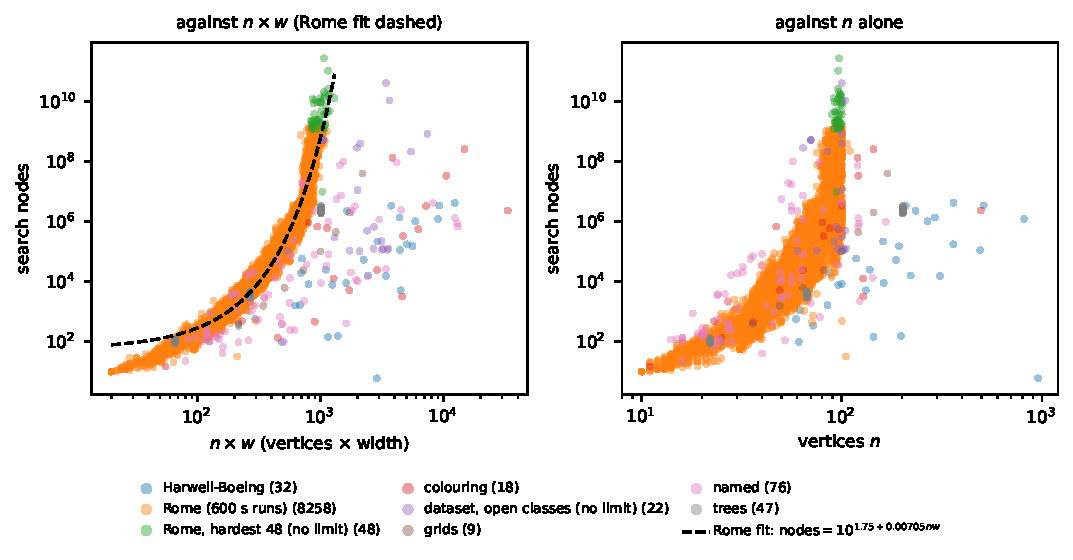
\includegraphics[width=\linewidth]{solve_times.pdf}
\caption{The cost of proving a pathwidth. Search nodes for every width our
search has proved (8,510 graphs, both axes logarithmic), against $n$ times the
width (left) and against $n$ alone (right). The dashed line is the fit on the
Rome graphs, $\text{nodes}=10^{1.75+0.00705\,nw}$. The structured benchmark
sets fall far below it, and size alone gives no single law.}
\label{fig:cost}
\end{figure}

\subsection{A checkable proof of a refutation}
\label{sec:certs}

A refutation by the search is a claim about a tree of up to $10^{12}$ nodes,
and Theorem~\ref{thm:main} proves the rules sound, not the code that runs
them. So the search emits a \emph{certificate}: the tree it explored, every
pruning step with its rule and its witness, and for each definite and better
step the matching of Theorem~\ref{thm:matching}. An independent checker, which
shares no code with the search, reads the instance matrix and the certificate.
At every node it checks that
\begin{itemize}
\item the premise of every pruning step holds, recomputed from the matrix;
\item every matching is valid: distinct customers, distinct stacks, each stack
  newly opened by its customer, and at least $\open-1$ edges;
\item every candidate within the bound is either a child or covered by a
  pruning step, and every chain of covers ends at a child or an old move,
  with no cycle;
\end{itemize}
and it replays the tree from the root. Each accepted step is a Lean theorem.
That an acyclic covering by such steps is sound is a short paper argument, not
yet a formal proof.

\begin{table}[t]
\centering\small
\caption{Every certificate the search emitted verifies, none is rejected, and
checking takes milliseconds. Certificates for our corrected rules, configuration
with better move, refuting the optimum minus one on the certified MOSP corpus
at 9--75 customers, with 60\,s to emit each. \emph{Not emitted}: the emitter
did not finish in time. Size is the compressed certificate; check time is the
independent checker's.}
\label{tab:certs}
\resizebox{\linewidth}{!}{% Generated by python -m paper1.latex.make_tables. Source: paper1/data/certificates/corrected.csv.
% Do not edit by hand.
\begin{tabular}{@{}lrrrrrr@{}}
\toprule
Customers & Instances & Verified & Rejected & Not emitted & Median size (bytes, gzip) & Median check (ms) \\
\midrule
9--10 & 1,614 & 1,614 & 0 & 0 & 332 & 0.04 \\
11--20 & 2,508 & 2,508 & 0 & 0 & 356 & 0.08 \\
21--30 & 1,816 & 1,816 & 0 & 0 & 414 & 0.24 \\
31--40 & 197 & 197 & 0 & 0 & 650 & 1.27 \\
41--50 & 120 & 120 & 0 & 0 & 12,045 & 33.24 \\
51--60 & 1 & 1 & 0 & 0 & 126,508 & 278.86 \\
61--75 & 30 & 19 & 0 & 11 & 26,516 & 143.70 \\
\bottomrule
\end{tabular}
% total csearch: 6275 of 6286 verified, 0 rejected, 35.47 MB gz, 147.4 s, 3353245 nodes
% total default: 6276 of 6286 verified, 0 rejected, 54.77 MB gz, 242.3 s, 5361282 nodes
}
\end{table}

Table~\ref{tab:certs} gives the results. Every refutation emitted within its
budget verifies, 6,275 of 6,286, and none is rejected. All 35.5\,MB of
certificates check in 147\,s. The base configuration gives the same picture:
6,276 of 6,286 verify and none is rejected. The checker also catches the error
of Section~\ref{sec:definite}. On the graph of
Counterexample~\ref{cex:definite}, rooted at $\{2\}$, the previous algorithm emits
a complete tree that claims there is no solution. A checker of the published
premises accepts it. Ours rejects it, even with a largest matching attached,
because the matching has one edge where two are needed. At 125 customers the
trees are too large to ship as certificates.

\subsection{A dataset with certified pathwidth}
\label{sec:dataset}

Section~\ref{sec:equiv} showed that one certified pathwidth $w$ answers every
problem in the exact core. Pathwidth, vertex separation and the vertex
separator game take the value $w$, and MOSP, gate matrix layout (which
multiple folding equals), one-dimensional logic, interval thickness,
narrowness, node search, progressive pebbling, the vertex search of
\citet{BRST1991} and the maximum wavefront take $w+1$: twelve problems in all, counting multiple folding with gate matrix layout. We therefore built one dataset from every benchmark collection of
those problems that we could obtain, including the MOSP corpus.

The unit of the dataset is the \emph{isomorphism class}: the set of instances
whose graphs are the same up to renaming the vertices. For a matrix instance
the graph is its MOSP graph. Two instances in one class have the same value
under every problem, so the dataset holds one record per class, with its
members and the renaming that maps each onto the record's graph. Classes were
found with nauty, a standard tool that computes a canonical form for each
graph. Each record carries the graph, the width $w$, its provenance, and a
witness layout of exactly that width. A record certified by bound also carries
a \emph{minor certificate}: a list of vertex deletions and edge contractions
after which every vertex has degree at least $w$. Any checker can replay it,
and it proves the pathwidth is at least $w$. A record certified on a minor
carries, when it is stored, the sequence of edge contractions that gives
the minor on which our search refuted width $w-1$, which proves $\pw\ge w$ by
Theorem~\ref{thm:minor}. A record certified by theorem names the theorem and
its Lean proof; so far these are the VSPLIB grids, whose pathwidth is given by
the grid theorem~\leanref{grid}.

\begin{table}[t]
\centering\small
\caption{Twenty collections, 21,754 instance files, reduce to 17,714
isomorphism classes, and 16,634 of them have a certified pathwidth with a
witness layout. Largely open: PACE, the VSPLIB Harwell--Boeing graphs, and the
MOSP sets of de Carvalho and Soma and of Frinhani et al. \emph{Classes}: isomorphism classes within the
collection (78 graphs above 5,000 vertices are compared by file content only).
\emph{Counted here}: classes whose first member, in the order of the table,
is in this collection, so the column sums to the dataset's class count. The
next six columns split those classes by provenance: certified by search on
the graph, by search on a contracted minor (Theorem~\ref{thm:minor}), by a
lower bound, or by a theorem; or an upper bound only. \emph{No witnessed
value}: no layout is stored yet; this includes one Rome class whose pathwidth
is certified but which has no stored layout of that width. $^{a}$The same 46 files distributed a second
time under other names; every class is counted under its first copy.}
\label{tab:dataset}
\resizebox{\linewidth}{!}{% Generated by python -m paper1.latex.make_tables. Source: paper1/data/dataset/{index,classes}.csv.gz.
% Do not edit by hand.
\begin{tabular}{@{}lrrrrrrrrr@{}}
\toprule
 & & & & \multicolumn{4}{c}{Certified} & & \\
\cmidrule(lr){5-8}
Collection & Files & Classes & Counted here & by search & on a minor & by bound & by theorem & Upper bound only & No witnessed value \\
\midrule
MOSP: Challenge 2005 & 5,806 & 3,169 & 3,169 & 3,168 & 0 & 1 & 0 & 0 & 0 \\
MOSP: Challenge 2005 (second copy)$^{a}$ & 46 & 46 & 0 & 0 & 0 & 0 & 0 & 0 & 0 \\
MOSP: Chu \& Stuckey & 200 & 200 & 200 & 200 & 0 & 0 & 0 & 0 & 0 \\
MOSP: Faggioli \& Bentivoglio & 300 & 287 & 274 & 274 & 0 & 0 & 0 & 0 & 0 \\
MOSP: SCOOP & 24 & 24 & 24 & 24 & 0 & 0 & 0 & 0 & 0 \\
VLSI gate matrix circuits & 11 & 11 & 11 & 5 & 0 & 5 & 0 & 1 & 0 \\
VSPLIB trees & 50 & 28 & 28 & 28 & 0 & 0 & 0 & 0 & 0 \\
VSPLIB grids & 50 & 50 & 50 & 9 & 0 & 0 & 41 & 0 & 0 \\
VSPLIB Harwell--Boeing & 73 & 72 & 72 & 32 & 5 & 7 & 0 & 28 & 0 \\
Small (Marti et al. 2008) & 84 & 84 & 84 & 32 & 0 & 52 & 0 & 0 & 0 \\
Rome graphs & 11,534 & 11,199 & 11,199 & 8,166 & 286 & 2,746 & 0 & 0 & 1 \\
TreewidthLIB colouring & 58 & 58 & 58 & 18 & 2 & 13 & 0 & 25 & 0 \\
freetdi named graphs & 150 & 146 & 143 & 103 & 1 & 22 & 0 & 16 & 1 \\
freetdi control-flow graphs & 1,817 & 1,070 & 1,064 & 398 & 2 & 661 & 0 & 2 & 1 \\
MOSP: Frinhani et al. 2018, large & 610 & 610 & 610 & 0 & 0 & 0 & 0 & 0 & 610 \\
PACE 2016 & 291 & 288 & 112 & 38 & 13 & 18 & 0 & 37 & 6 \\
PACE 2017 exact & 200 & 199 & 193 & 61 & 61 & 7 & 0 & 54 & 10 \\
PACE 2017 heuristic & 200 & 197 & 173 & 11 & 5 & 3 & 0 & 40 & 114 \\
PACE 2017 bonus & 100 & 100 & 100 & 24 & 54 & 0 & 0 & 22 & 0 \\
MOSP: Carvalho \& Soma 2015 & 150 & 150 & 150 & 38 & 0 & 0 & 0 & 112 & 0 \\
\midrule
All & 21,754 &  & 17,714 & 12,629 & 429 & 3,535 & 41 & 337 & 743 \\
\bottomrule
\end{tabular}
}
\end{table}

Table~\ref{tab:dataset} gives the counts. The collections are the MOSP
collections
\citep{SmithGent2005,FaggioliBentivoglio1998,ChuStuckey2009,CarvalhoSoma2015,Frinhani2018},
eleven VLSI gate matrix circuits \citep{OliveiraLorena2002}, the VSPLIB sets
\citep{Duarte2012} and the Small graphs \citep{MartiCamposPinana2008}, the Rome
graphs \citep{DiBattista1997}, and treewidth collections used as pathwidth
benchmarks \citep{TreewidthLIB,freetdi,PACE2016,PACE2017}. Of the 17,714
classes, 16,634 carry a certified pathwidth with a witness layout and 337 a witnessed upper bound, and 743 have no witnessed value yet, one of them with a certified pathwidth. The 610 large instances of \citet{Frinhani2018}, with
400 to 1,000 customers, are included so that the dataset covers every
published MOSP collection we have. None of them has a value yet, because an
exact search at that size is out of reach.

An independent checker, sharing no code with the solvers, verifies the
dataset. It re-reads all 20,984 member files with its own readers, maps each
onto its record's graph by its renaming, recomputes the width of every witness
layout, replays every minor certificate and every stored contraction sequence
(424 of the 429 records certified on a minor), and recognises each grid
certified by theorem from its edges alone. It reports no failure on the
16,971 records, the 16,634 certified classes and the 337 with an upper bound. A value certified by search cannot be checked from its record,
and neither can the refutation on a minor;
both rest on our corrected search, and for instances within reach of the emitter
the certificate of Section~\ref{sec:certs} is how a third party can check it.

\paragraph{Agreement with published values.} All 84 Small graphs agree with
the pathwidths of \citet[Tables~4--5]{Mallach2018}. Ten of the eleven VLSI
circuits are certified at their published best-known track counts
\citep[Table~I]{OliveiraLorena2002}; the eleventh, W4 with 202 nets, is open
at 28 against 27.

\paragraph{A caution about MOSP files.} A MOSP file can be read with rows as
customers or with rows as patterns, and the two readings give different
graphs. The same public repository ships the
\citet{CarvalhoSoma2015} instances as customers by patterns and the
\citet{ChuStuckey2009} instances beside them as patterns by customers. Only
published densities and values tell them apart. Read the wrong way round, an
instance certifies at a different value.
